\section{Optimal Control of Pitch and Travel without Feedback}\label{sec:prob2}

In this section we compute an optimal trajectory $x^*$ and a corresponding input sequence $u^*$. The trajectory should bring the helicopter from an initial state to a desired final state. We do not use feedback to correct for deviations from the calculated trajectory. The computation of the optimal trajectory was formulated as a convex optimization problem.

\subsection{The helicopter model on continuous-time state-space form}
The system (\ref{eq:model_al}) describes the helicopter plant, with a basic control layer consisting of PID and PD controllers for elevation and pitch. In this section we focus on the optimization layer that gives the input to these regulators, see figure (\ref{fig:control_hierarchy}).
\begin{figure}[ht]
    \centering
    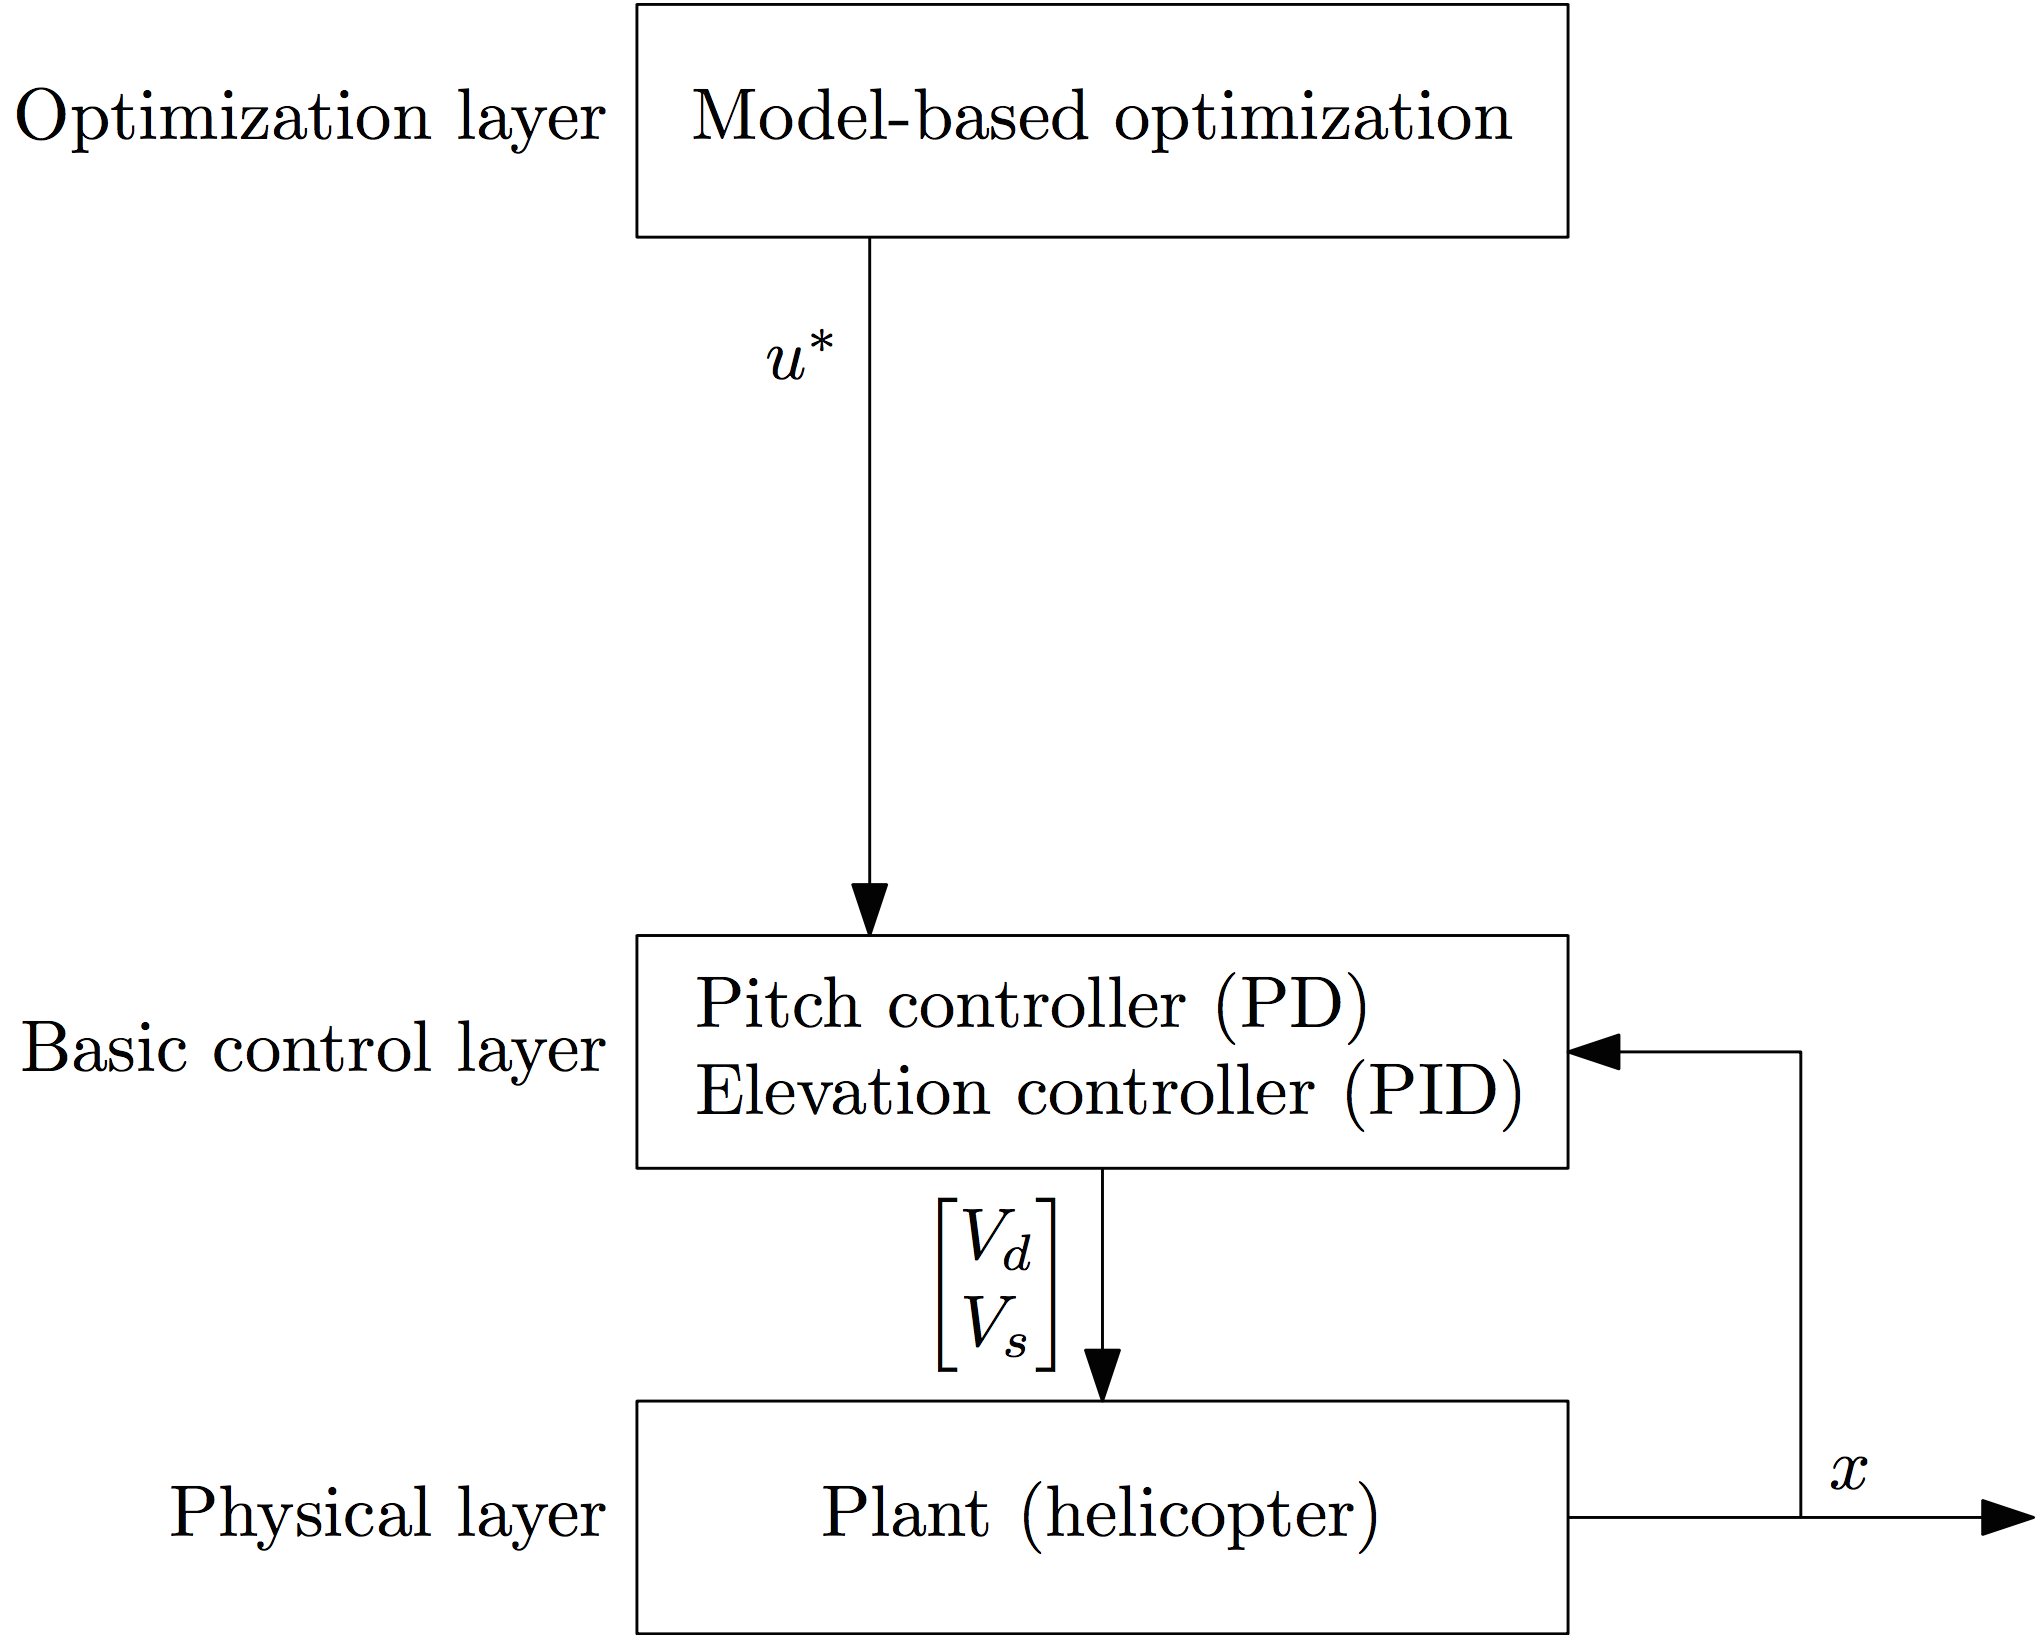
\includegraphics[width=0.6\textwidth]{figures/day2/control_hierarchy_day2}
    \caption{Control hierarchy}
    \label{fig:control_hierarchy}
\end{figure}
Throughout this section we will disregard elevation, that is, we assume $e = 0$.
The system can then be written on the continuous-time state-space form:
\begin{equation}
    \dot{x} = A_cx + B_cu
    \label{eq:state_space_axbu}
\end{equation}
with $x = \begin{bmatrix} \lambda & r & p & \dot{p} \end{bmatrix}^T$ and $u = p_c$.
The continuous-time system matrices for this model are:
\begin{equation}
    A_c = \begin{bmatrix} 0 & 1 & 0 & 0 \\ 0 & 0 & -K_2 & 0 \\ 0 & 0 & 0 & 1 \\ 0 & 0 & -K_1K_{pp} & -K_1K_{pd} \end{bmatrix}
    \qquad\text{and}\qquad
    B_c = \begin{bmatrix}0 \\ 0 \\ 0 \\K_1K_{pp} \end{bmatrix}
\end{equation}

\subsection{Discretization}

The system dynamics is implemented as a sequence of constraints in the
optimization problem, and must therefore be written in discrete-time state-
space form,
\begin{equation}
    x_{k+1} = Ax_k + Bu_k.
    \label{eq:discrete_state_space_axbu}
\end{equation}
We discretize the model using the Euler method, by approximating derivatives
with a forward difference over a timestep $h$:
\begin{equation}
    \dot{x}_k \approx \frac{x_{k+1} - x_k}{h}
\end{equation}
Inserting this into (\ref{eq:state_space_axbu}), we obtain
\begin{equation}
    x_{k+1} \approx (I + hA_c) x_k + hB_c u_k
\end{equation}
A suitable approximation for the discrete-time matrices is then
\begin{equation}
    A \approx I + hA_c
    \qquad\text{and}\qquad
    B \approx hB_c
\end{equation}

\subsection{Computation of optimal trajectory}

An optimal trajectory can be generated by minimizing the cost function
\begin{equation}
    \label{eq:trajectory_cost}
    \phi = \sum_{i=1}^{N}(\lambda_i - \lambda_f)^2 + qp_{ci}^2
\end{equation}
for some scalar weight $q \geq 0$ over the finite horizon of states and inputs

\begin{equation}
    z = (x_1 \; x_2 \; ... \; x_N \; u_1 \; u_2 \; ... \; u_N)^T
\end{equation}

subject to various equality and inequality constraints. The discrete system dynamics are implemented as equality constraints of the form $A_{\text{eq}}z = B_{\text{eq}}$, where $A_{\text{eq}}$ and $B_{\text{eq}}$ are given by the left- and right-hand side of the $N$ constraints
\begin{align*}
    x_1 - Bu_0        &= Ax_0 \\
    x_2 - Ax_1 - Bu_1 &= 0    \\
    \vdots                    \\
    x_N - Ax_{N-1} - Bu_{N-1} &= 0
\end{align*}

We would also like to constrain the system state and input to be within a range

\begin{align}
    x^{\text{min}} \leq x_{t+1} \leq x^{\text{max}} \\
    u^{\text{min}} \leq u_t \leq u^{\text{max}}
\end{align}

for $t = 0...N-1$. Applying these constraints to all states and inputs in the solution horizon, we have
\begin{equation}
    \begin{bmatrix} I \\ -I \end{bmatrix} z
    \leq
    \begin{bmatrix}
    \{x_{t+1}^{max}\} \\
    \{u_t^{max}\} \\
    \{x_{t+1}^{min}\} \\
    \{u_t^{min}\}
    \end{bmatrix}_{t=0..N-1}
\end{equation}
which can be implemented as an inequality constraint of the form $A_{\text{iq}} z \leq B_{\text{iq}}$. Together, these equations form a quadratic optimization problem, which can be readily solved by efficient techniques.

The cost function (\ref{eq:trajectory_cost}) balances how much we wish to penalize state error, $(\lambda_i - \lambda_f)^2$, and the conservation of input. By increasing the value of $q$, the optimal trajectory will tend to keep the pitch setpoint $p_c$ small, while allowing for potentially larger state error. A small value of $q$ will make the state error relatively more expensive, and allow the trajectory to use large pitch angles to bring the error to zero quickly.

Note that the cost function does not take into consideration that $\lambda_i$ plus some multiple of $2\pi$ describes the same physical orientation of the helicopter. For example, if the reference is $0$ and $\lambda_i = 2\pi$, it will be regarded as a large error, even though the helicopter is in fact in the desired orientation. A more optimal scheme would take this into consideration.

\subsection{Results}

We solved the optimization problem using the built-in MATLAB function \texttt{quadprog}. The result was a simulated state trajectory, and the corresponding optimal input sequence. We fed the input sequence directly into the internal regulators, as shown in figure (\ref{fig:day2_mdl}). Zeroes were added on both sides of the input sequence to give time to initialize and stabilize the helicopter.

\begin{figure}[htb]
    \centering
        \makebox[\textwidth][c]{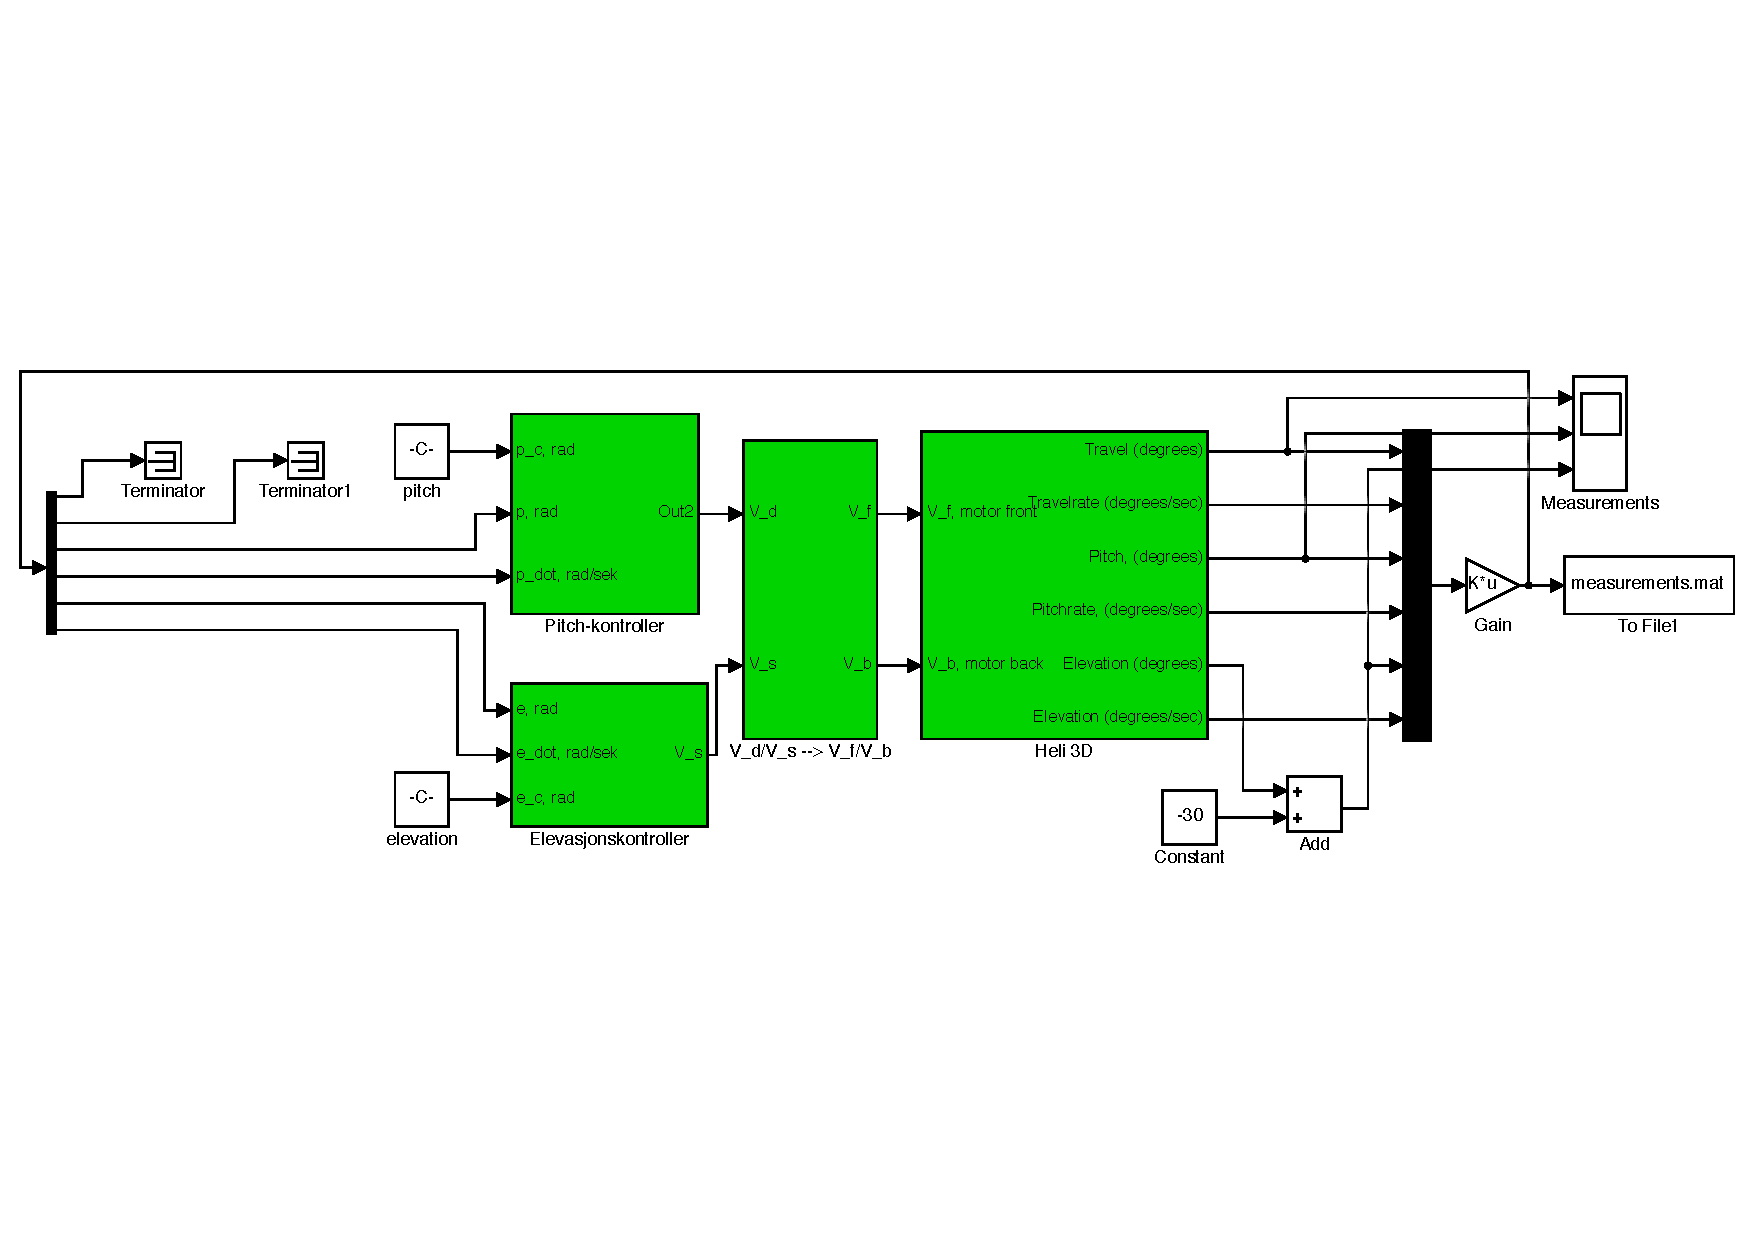
\includegraphics[width=\textwidth]{figures/day2/day2_mdl}}
    \caption{Plot of day 2}
    \label{fig:day2_mdl}
\end{figure}

Figure (\ref{fig:day2_plot}) shows the measured trajectories for travel and pitch, using $q = 1$. We see that the helicopter did not reach the planned final state, even though the pitch matched fairly well with the optimal setpoint. Selecting different values of $q$ did not lead to any significant improvements, and the helicopter still deviated heavily from the planned trajectory.

The biggest cause for this is the lack of feedback. Modelling inaccuracies, disturbances, and linearization errors all contribute to the computed input being unfit for the real system. Since constructing a perfect model is unrealistic, feedback is necessary compensate for such errors.

\begin{figure}[htb]
    \centering
        \makebox[\textwidth][c]{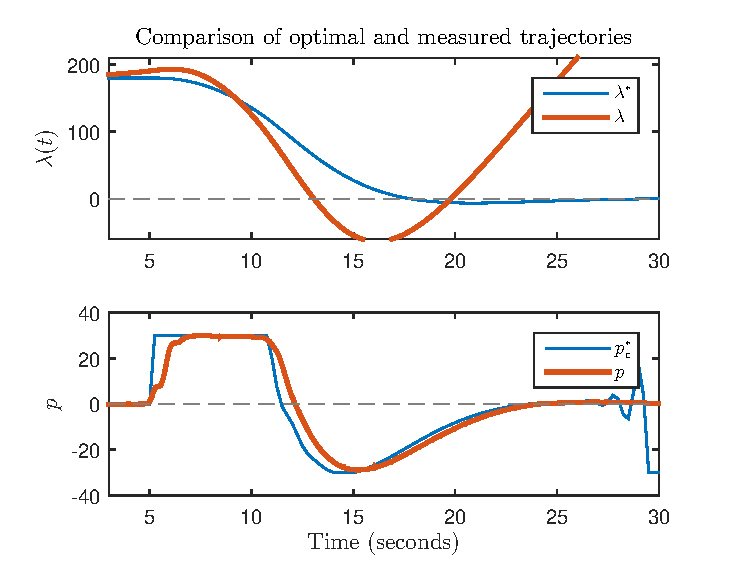
\includegraphics[width=\textwidth]{figures/day2/plot_day2}}
    \caption{Plot of day 2}
    \label{fig:day2_plot}
\end{figure}
